\Transcb{yellow}{blue}{Introduction}
\onecolumn
\begin{itemize}
\item Observations in the neighbourhood of our solar system and galaxy
\item[] Concentrations of matter (Sun, planets, stars,...) and  rather empty regions
\item[] Things look different in different directions (e.g. galactic plane and celestial poles)
\end{itemize}
%
\begin{center}
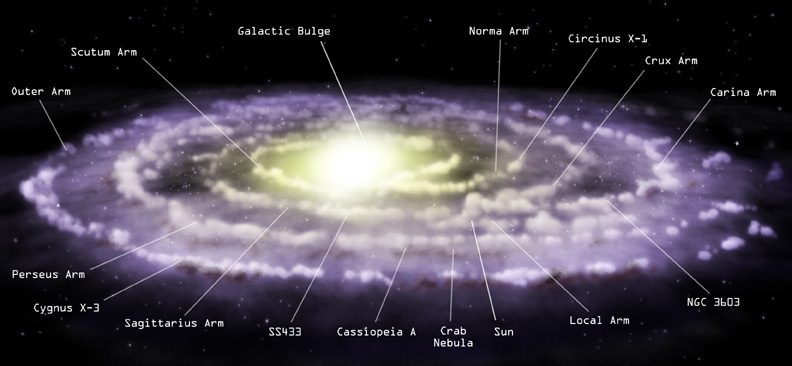
\includegraphics[keepaspectratio,width=25cm]{milky-way}
\end{center}

\Tr
\onecolumn
\begin{itemize}
\item Somewhat larger scale : Clusters of galaxies $\rightarrow$ structures of stars etc... disappear
\item[] Still a bit "clumpy" but things start to look the same in whatever direction one looks
\end{itemize}
%
\begin{center}
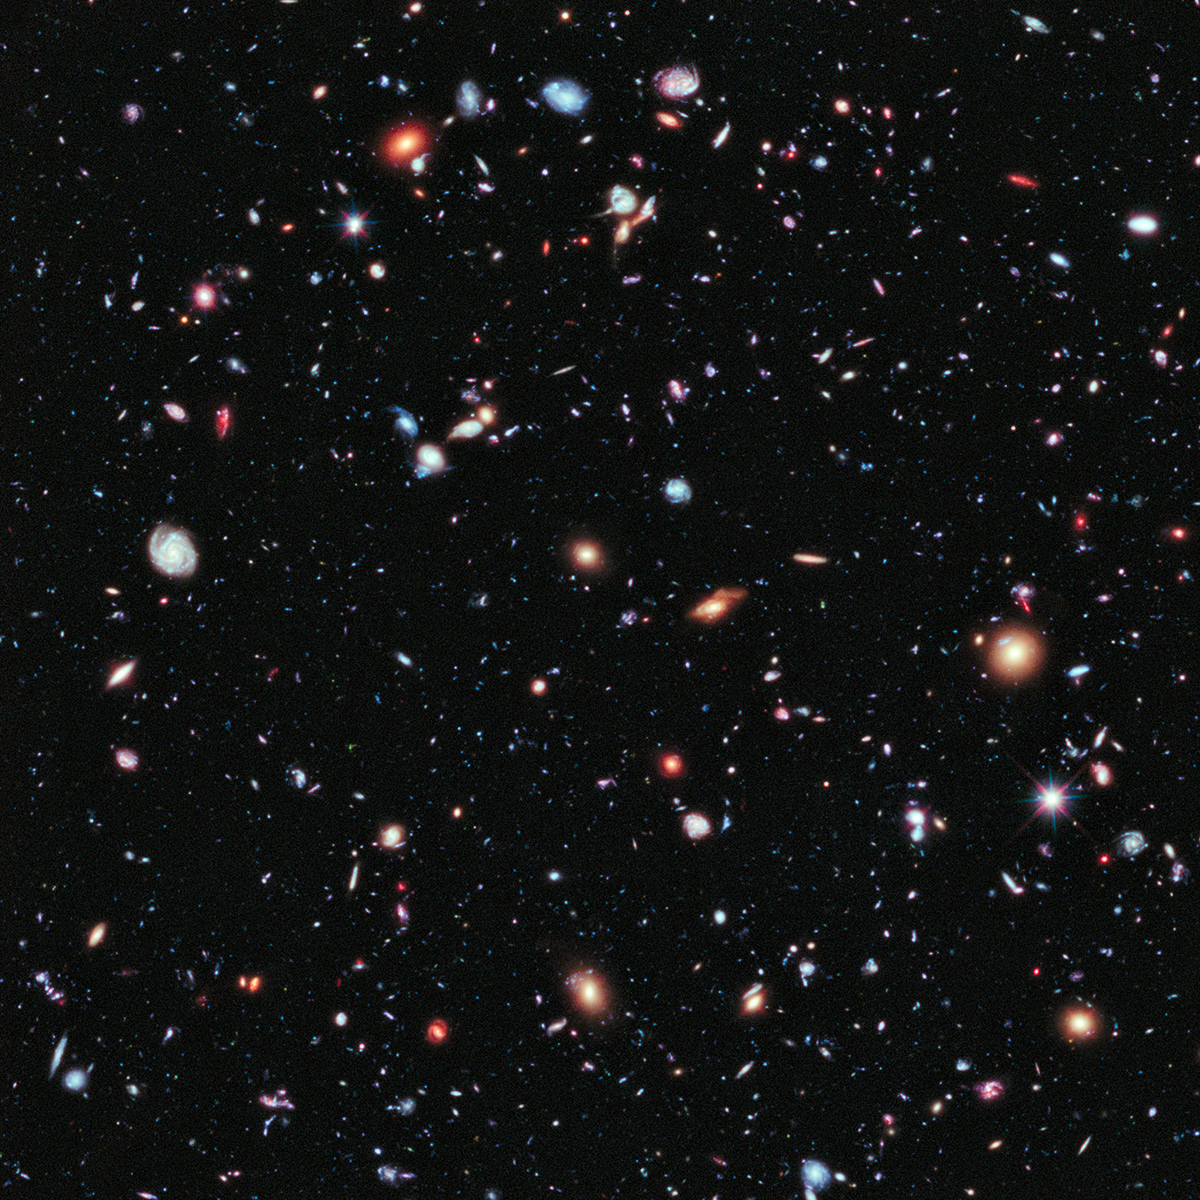
\includegraphics[keepaspectratio,height=12.5cm]{galaxies}
\end{center}

\Tr
\onecolumn
\begin{itemize}
\item Quantitative investigation of the structure of the universe
\item[] Consider spheres with radius $R$ and place them at random locations in the universe
\item[] Determine the energy (incl. mass) density $\rho_{i}$ within each sphere
\item[] Calculate the average density $\bar{\rho}$ from all these spheres
\item[] Observation~: fractional density fluctuations
        $(\rho_{i}-\bar{\rho})/\bar{\rho} \propto R^{-\alpha} \qquad (\alpha>0)$
\item[$\ast$] At very large scales : Uniform density $\rightarrow$ {\blue homogeneous} universe
\item[] Random placement of our test sphere $\rightarrow$ Same observations from any location
\item[$\ast$] At very large scales the universe becomes {\blue isotropic}
\item Large Scale Universe can be described as a {\red cosmic fluid} and we are part of it
\item[] {\blue How to describe the space-time structure (metric) of this cosmic fluid ?}
\end{itemize}
